%
% compmod.tex -- Beispiel zum computational mode
%
% (c) 2018 Prof Dr Andreas Müller, Hochschule Rapperswil
%
\documentclass[tikz]{standalone}
\usepackage{times}
\usepackage{txfonts}
\usepackage[utf8]{inputenc} 
\usepackage{graphics}
\usepackage{ifthen}
\usepackage{color}
\usetikzlibrary{arrows,intersections}
\usetikzlibrary{math}
\begin{document} 
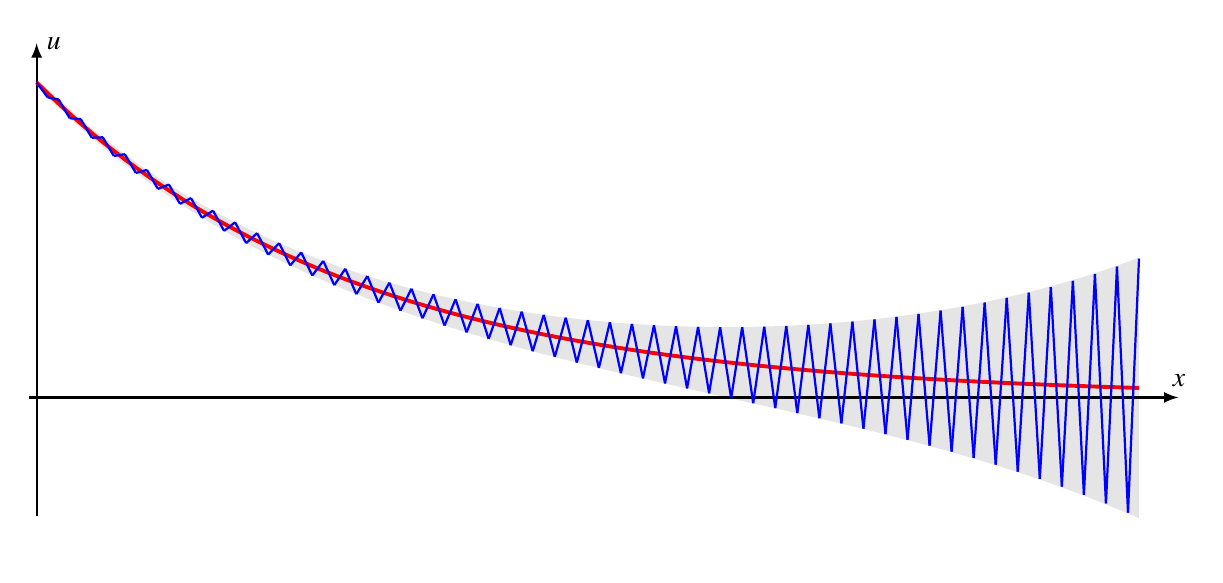
\begin{tikzpicture}[>=latex,thick]
\begin{scope}
\clip (0,-2) rectangle (14,4);
\fill[color=gray!20]
	plot[domain=0:14,samples=100] ({\x},{4*exp(-\x/4)-0.05*exp(\x/4)})
	--
	plot[domain=14:0,samples=100] ({\x},{4*exp(-\x/4)+0.05*exp(\x/4)})
	--cycle;
\end{scope}
\draw[->] (-0.1,0)--(14.5,0) coordinate[label=$x$];
\draw[->] (0,-1.5)--(0,4.5) coordinate[label={right:$u$}];
\draw[color=red,line width=1.4pt]
	plot[domain=0:14,samples=100] ({\x},{4*exp(-\x/4)});

\tikzmath{
	real \h, \N;
	\N = 100;
	\h = 14/\N;
	real \x, \xalt, \ualt;
	\xalt = 0;
	\ualt = 4;
	real \lambdaminus, \lambdaplus;
	\lambdaplus = sqrt(1 + \h*\h/16)-\h/4;
	\lambdaminus = -sqrt(1 + \h*\h/16)-\h/4;
	real \aplus, \aminus;
	\aplus = 4;
	\aminus = 0.05;
	real \uminus, \Uplus;
	\Uplus = \aplus;
	\uminus = \aminus;
}

\foreach \i in {1,2,...,\N}{
	\pgfmathparse{\xalt+\h}
	\xdef\x{\pgfmathresult}
	\pgfmathparse{\Uplus * \lambdaplus}
	\xdef\Uplus{\pgfmathresult}
	\pgfmathparse{\uminus * \lambdaminus}
	\xdef\uminus{\pgfmathresult}
	\draw[color=blue] ({\xalt},{\ualt})--({\x},{\Uplus+\uminus});
	\xdef\xalt{\x}
	\pgfmathparse{\Uplus+\uminus}
	\xdef\ualt{\pgfmathresult}
}
\end{tikzpicture}
\end{document}
